% =====================================================================
% TCC no formato SBC (modelo da Unit: tcc/modelo-tcc-sbc.tex)
% Compilar duas vezes: pdflatex tcc-afora-sbc.tex
% =====================================================================
\documentclass[a4paper,12pt]{article}

\usepackage[utf8]{inputenc}
\usepackage[T1]{fontenc}
% Português: com babel quando o pacote existe (TeX Live completo). Sem ele,
% os nomes são definidos à mão e a hifenização é desligada, para não hifenizar
% palavras portuguesas com padrões do inglês.
\IfFileExists{brazil.ldf}{\usepackage[brazilian]{babel}\newif\ifptbabel\ptbabeltrue}{%
  \newif\ifptbabel\ptbabelfalse}
\usepackage{microtype}
\usepackage{times}
\usepackage[a4paper,top=3.5cm,left=3cm,right=3cm,bottom=2.5cm]{geometry}
\usepackage{graphicx}
\usepackage{url}
\expandafter\def\expandafter\UrlBreaks\expandafter{\UrlBreaks\do\-}
\usepackage{indentfirst}
\usepackage{titlesec}
\usepackage[bf,sf,footnotesize,indent]{caption}
\usepackage{array}
\usepackage{tabularx}
\usepackage{booktabs}
\usepackage{listings}
\usepackage{xcolor}
\usepackage[authoryear,round,semicolon]{natbib}
% ABNT: \citep com o nome em maiúsculas; citações narrativas escritas como "Nome (\citeyear{chave})"
\providecommand{\NoCaseChange}[1]{#1} % TeX Live anterior a 2022 não define
\DeclareRobustCommand{\etal}{\NoCaseChange{\textit{et al.}}}
\makeatletter
\def\NAT@nmfmt#1{{\MakeUppercase{#1}}}
\makeatother

\setlength{\parindent}{1.27cm}
\setlength{\parskip}{6pt}
\raggedbottom

\titleformat{\section}{\fontsize{13}{15}\bfseries}{\thesection.}{1em}{}
\titleformat{\subsection}{\fontsize{12}{14}\bfseries}{\thesubsection.}{1em}{}
\titleformat{\subsubsection}{\fontsize{12}{14}\bfseries\itshape}{\thesubsubsection.}{1em}{}
\titlespacing*{\section}{0pt}{12pt}{6pt}
\titlespacing*{\subsection}{0pt}{10pt}{4pt}

\renewcommand{\captionfont}{\sffamily\footnotesize\bfseries}
\setlength{\captionmargin}{0.8cm}
\captionsetup{labelsep=period}
\captionsetup[table]{skip=4pt}

\newenvironment{resumo}{%
  \list{}{\advance\topsep by6pt\relax
    \leftmargin=0.8cm
    \labelwidth=0pt
    \listparindent=0pt
    \itemindent\listparindent
    \rightmargin\leftmargin}\item[\hskip\labelsep\bfseries\itshape Resumo.]\itshape}%
  {\endlist}

\renewenvironment{abstract}{%
  \list{}{\advance\topsep by6pt\relax
    \leftmargin=0.8cm
    \labelwidth=0pt
    \listparindent=0pt
    \itemindent\listparindent
    \rightmargin\leftmargin}\item[\hskip\labelsep\bfseries\itshape Abstract.]\itshape}%
  {\endlist}

% Listagens de código: legenda "Listagem N." acima, sem quebra de página
\renewcommand{\lstlistingname}{Listagem}
\lstdefinelanguage{TypeScript}{
  keywords={import,from,export,class,extends,const,private,public,static,return,new,get,void,string,implements,constructor,readonly,type},
  sensitive=true, comment=[l]{//}, morestring=[b]", morestring=[b]'}
\lstset{language=TypeScript, basicstyle=\ttfamily\footnotesize, columns=fullflexible,
  keepspaces=true, keywordstyle=\bfseries, commentstyle=\itshape\color{black!60},
  frame=lines, framesep=4pt, xleftmargin=6pt, xrightmargin=6pt,
  captionpos=t, abovecaptionskip=4pt, belowcaptionskip=4pt, upquote=true,
  literate={á}{{\'a}}1 {é}{{\'e}}1 {í}{{\'i}}1 {ó}{{\'o}}1 {ú}{{\'u}}1 {ç}{{\c{c}}}1 {ã}{{\~a}}1 {õ}{{\~o}}1 {ê}{{\^e}}1 {Ç}{{\c{C}}}1}

% Floats grandes (listagens) podem dividir a página com o texto
\renewcommand{\topfraction}{0.85}\renewcommand{\textfraction}{0.1}\renewcommand{\floatpagefraction}{0.8}

% Fonte de figuras e tabelas
\newcommand{\fonte}[1]{\par\vspace{2pt}{\centering\sffamily\footnotesize Fonte: #1\par}}
% Termos estrangeiros não dicionarizados
\newcommand{\estr}[1]{\textit{#1}}

\ifptbabel\else
  \renewcommand{\figurename}{Figura}\renewcommand{\tablename}{Tabela}
  \renewcommand{\refname}{Referências}\renewcommand{\contentsname}{Sumário}
  \hyphenpenalty=10000 \exhyphenpenalty=10000
  \emergencystretch=3em
\fi
\begin{document}
\pagestyle{empty}

\begin{center}
  {\fontsize{16}{20}\selectfont\bfseries Da cerimônia à declaração: o afora e as garantias de \textit{runtime} para \textit{backends} TypeScript escritos por pessoas e agentes de IA}\\[4pt]
  {\fontsize{14}{18}\selectfont\bfseries From ceremony to declaration: afora and runtime guarantees for TypeScript backends written by people and AI agents}\\[12pt]

  {\normalsize\bfseries Alan Reis Anjos$^{1}$, Luiz Gomes da Cunha Neto$^{1}$}\\[6pt]

  {\normalsize
    $^{1}$Ciência da Computação -- Universidade Tiradentes\\{}
    Aracaju, Sergipe -- SE\\{}
    \footnotesize\texttt{alan.reis@souunit.com.br, alan.reis@getafora.com, luiz\_gomes@unit.br}
  }
\end{center}
\vspace{12pt}

\begin{resumo}
Agentes de IA barateiam a produção de código e encarecem a sua revisão; o conteúdo de baixa qualidade gerado em massa ganhou o nome de \textit{AI slop}. Este trabalho apresenta o afora, um \textit{framework} de código aberto para \textit{backends} em TypeScript, construído em três gerações segundo a Design Science Research. Quem escreve a aplicação, pessoa ou agente, declara o modelo do domínio, e o \textit{runtime} mantém invariantes genéricas: algumas por padrão, como a rejeição de campos não declarados, e outras a partir de declarações, como a unicidade e o controle de acesso. Um CRUD padrão coube em 3,6 vezes menos caracteres que uma versão enxuta em Hono e Zod; numa API real com regras próprias, porém, o código cresceu 27\% e mudou de lugar. Numa avaliação de viabilidade, com uma execução por lado, um agente construiu um \textit{backend} só pelo servidor MCP do afora e manteve as cinco garantias verificadas sem código de implementação; a linha de base, escrita pelo mesmo agente, também as manteve. Conclui-se que o afora preserva, por construção, as invariantes que declara; se isso reduz as falhas de agentes fica para uma avaliação em lote, já instrumentada.
\end{resumo}
\noindent\textbf{Palavras-chave:} \textit{AI slop}; agentes de IA; Domain-Driven Design; \textit{frameworks}; TypeScript.

\vspace{6pt}

\begin{abstract}
AI agents make code cheap to produce and expensive to review; the low-quality content they mass-produce has been named AI slop. This work presents afora, an open-source framework for TypeScript backends, built in three generations following Design Science Research. Whoever writes the application, person or agent, declares the domain model, and the runtime keeps generic invariants: some by default, such as rejecting undeclared fields, and others from declarations, such as unique keys and access control. A standard CRUD took 3.6 times fewer characters than a lean Hono and Zod version; in a real API with its own rules, however, the code grew 27\% and changed place. In a feasibility evaluation with one run per side, an agent built a backend solely through afora's MCP server and kept the five checked guarantees with no implementation code; the baseline the same agent wrote kept them too. We conclude that afora preserves by construction the invariants it declares; whether this reduces agent failures is left to a batch evaluation that is already instrumented.
\end{abstract}
\noindent\textbf{Keywords:} AI slop; AI agents; Domain-Driven Design; frameworks; TypeScript.

\vspace{12pt}

% =====================================================================
\section{Introdução}\label{sec:intro}

Em fevereiro de 2025, Karpathy (\citeyear{karpathy2025}) chamou de \estr{vibe coding} a prática de pedir a um modelo de linguagem que escreva um programa e aceitar o resultado sem ler o código. Produzir software ficou muito mais barato, e produzir software ruim ficou mais barato ainda. O nome que se consolidou para o produto dessa segunda tendência é \estr{AI slop}: conteúdo gerado em quantidade, sem cuidado, que custa a quem o recebe mais do que custou a quem o gerou.

\estr{Backends} HTTP são um terreno fértil para esse tipo de falha. Um \estr{backend} correto precisa de garantias que não aparecem na especificação funcional: o \estr{hash} da senha não pode sair numa resposta, campos que o cliente não deveria enviar precisam ser recusados, um e-mail único não pode ser gravado duas vezes, um erro de negócio não pode virar HTTP~500, e um usuário não pode ler os dados de outro. Em \estr{frameworks} convencionais, cada uma dessas garantias é uma convenção: um \texttt{.strict()} num \estr{schema}, um filtro antes da resposta, uma checagem em cada rota. Convenções dependem de memória, e memória é o que falha quando o código é escrito às pressas, por uma pessoa ou por um agente. A resposta usual é revisar mais, mas a revisão é justamente o recurso escasso.

O problema deste trabalho é, portanto: \textbf{como projetar um \estr{framework} de \estr{backend} em que um conjunto de invariantes genéricas da API seja mantido pelo \estr{runtime}, e não pelo código da aplicação, e o que isso muda no que pessoas e agentes de IA precisam escrever e revisar?} A resposta proposta tem dois níveis. Algumas garantias valem por padrão: não há linha da aplicação que as ligue, e por isso não há onde esquecê-las. Outras dependem de uma declaração, como dizer que um campo é único ou quem é o dono de um recurso; essas ainda podem ser esquecidas, mas num único lugar, o modelo, que se revisa lendo declarações e não implementações.

O objetivo geral é desenvolver e avaliar um \estr{framework} para \estr{backends} em TypeScript que mantenha no \estr{runtime} invariantes de segurança e consistência de uma API, e medir o que isso muda no código que se escreve e se revisa. Os objetivos específicos são: (1) identificar as garantias que um \estr{backend} tende a perder quando escrito sem cuidado; (2) projetar um modelo de declaração único, a \estr{blueprint}, do qual se derivem entidade, validação, repositório e contrato HTTP; (3) implementar essas garantias como comportamento do \estr{runtime}; (4) oferecer a aplicação como dados e uma interface para agentes via Model Context Protocol (MCP); e (5) avaliar o produto quanto ao volume de código, à viabilidade de um \estr{backend} construído por agente, ao custo de revisão e ao desempenho. Detalhes de medição, histórico e uso real que este artigo resume estão no relatório técnico do trabalho \citep{anjos2026tcc}.

% =====================================================================
\section{Fundamentação Teórica e Trabalhos Relacionados}\label{sec:fund}

\subsection{\textit{AI slop} e código gerado por IA}\label{sec:slop}

Willison (\citeyear{willison2024}) popularizou \estr{slop} como o equivalente, para o conteúdo de IA indesejado, do que \estr{spam} é para o e-mail. O traço que o define é a assimetria de esforço: exige mais para consumir do que exigiu para produzir. No software, o caso mais documentado é o do curl, cujo mantenedor passou, em maio de 2025, a banir quem enviasse relatórios de segurança considerados \estr{slop} \citep{newstack2026} e, em janeiro de 2026, encerrou o programa de recompensas mantido desde 2019 \citep{stenberg2026}: o custo de produzir um relatório caiu para quase zero, e o de verificá-lo continuou humano.

Os efeitos sobre a produtividade são controversos, e os estudos mais citados ainda são \estr{preprints}: um experimento mediu tarefas 55,8\% mais rápidas com o GitHub Copilot \citep{peng2023}, e um ensaio randomizado com desenvolvedores experientes mediu tarefas 19\% mais lentas com IA, embora os participantes se julgassem mais rápidos \citep{becker2025}. Os efeitos sobre a qualidade, nos estudos revisados por pares, são mais consistentes. Cerca de 40\% dos programas gerados pelo Copilot em cenários ligados a vulnerabilidades conhecidas eram vulneráveis \citep{pearce2022}; usuários com assistente escreveram código menos seguro e se julgaram mais seguros \citep{perry2023}; e, no BaxBench, cerca de metade dos \estr{backends} funcionalmente corretos gerados por cada modelo podia ser explorada \citep{vero2025}. O defeito está no que não aparece à primeira leitura, que num \estr{backend} são as garantias implícitas da Seção~\ref{sec:intro}.

\subsection{Bases do projeto}

O afora se apoia em quatro tradições. Do Domain-Driven Design \citep{evans2004} e da Clean Architecture \citep{martin2018}, herda o modelo de domínio no centro e a regra de dependência, cujo preço é a complexidade acidental \citep{brooks1987}: classes, interfaces, fábricas e \estr{mappers} que repetem a mesma estrutura para cada conceito. Da engenharia dirigida por modelos, herda a ideia de gerar código a partir de um modelo, e a crítica de que modelo e código divergem ao primeiro ajuste manual \citep{hailpern2006}. Das bibliotecas de validação em tempo de execução, necessárias porque os tipos do TypeScript não existem após a compilação, herda o princípio \estr{parse, don't validate} \citep{king2019}: a validação deve produzir um valor de tipo mais preciso, e não apenas aprovar a entrada. As propriedades do afora são construídas sobre o TypeBox \citep{typebox2026}, que cria \estr{schemas} JSON Schema inferidos como tipos do TypeScript e os compila em validadores. Da segurança de APIs, adota as categorias da OWASP API Security Top 10 \citep{owasp2023} e o formato \texttt{problem+json} da RFC 9457 \citep{rfc9457} para erros.

\subsection{Análise de similares}\label{sec:similares}

Foram comparados o NestJS, a combinação Hono + Zod (linha de base da avaliação), o tRPC e o Ruby on Rails. O critério não é o que cada ferramenta permite, mas o que garante por padrão, sem que o desenvolvedor escreva ou configure nada: essa é a pergunta relevante quando o código é escrito por um agente que pode esquecer a configuração (Tabela~\ref{tab:similares}). As células marcadas com \textsuperscript{b} foram conferidas com projetos mínimos: um cadastro que devolve a entidade com o \estr{hash}, uma requisição com a chave extra \texttt{isAdmin} e um e-mail repetido sinalizado por um \texttt{Error} comum.

\begin{table}[ht]
\centering
\caption{Garantias oferecidas por padrão pelas ferramentas analisadas.}\label{tab:similares}
\scriptsize
\setlength{\tabcolsep}{4pt}
\renewcommand{\arraystretch}{1.12}
\begin{tabularx}{\linewidth}{>{\raggedright\arraybackslash}p{2.0cm}*{5}{>{\raggedright\arraybackslash}X}}
\toprule
Garantia & NestJS & Hono + Zod & tRPC & Rails & afora \\
\midrule
Campos não declarados recusados & Aceitos no padrão; recusados só com duas opções\textsuperscript{a,b} & Removidos; recusados com \texttt{.strict()} e validador, 500 sem ele\textsuperscript{b} & Removidos; recusados com \texttt{z.strictObject}\textsuperscript{b} & Filtrados por \estr{strong parameters} em cada controlador & Recusados em qualquer profundidade (400) \\
Dados sensíveis fora das respostas & Vazam; ocultos só com \texttt{@Exclude} e o interceptor\textsuperscript{b} & Manual\textsuperscript{b} & Manual\textsuperscript{b} & Manual & Mascarados pelo \texttt{toJSON()}\textsuperscript{c} \\
Chaves únicas & Banco ou código & Manual & Manual & Validação de modelo, sujeita a duplicatas sem índice & Garantidas pelo repositório (409)\textsuperscript{c} \\
Erro de negócio com status correto & \texttt{Error} comum vira 500\textsuperscript{b} & Manual (\texttt{onError})\textsuperscript{b} & \texttt{Error} comum vira 500\textsuperscript{b} & Parcial & Por camada, em \texttt{problem+json} \\
Acesso por dono & \estr{Guards} por rota & Manual & \estr{Middlewares} & Manual por controlador & Declarado no caso de uso\textsuperscript{c} \\
Aplicação como dados para agentes & Não & Não & Não & Não & \texttt{afora.json} e MCP \\
\bottomrule
\end{tabularx}
\fonte{elaborado pelo autor com base na documentação oficial (nov. 2026) \citep{nestjs2026,zod2026,rails2026}. \textsuperscript{a}\texttt{whitelist} e \texttt{forbidNonWhitelisted}. \textsuperscript{b}Conferido com projeto mínimo em 22/11/2026 (\path{tcc/metrics/similares/}). \textsuperscript{c}Vale para o que o modelo declara; a senha é sensível por padrão (Tabela~\ref{tab:garantias}).}
\end{table}

A tabela não diz que as alternativas sejam inseguras: cada comportamento muda com uma linha de configuração ou de código, e um time disciplinado mantém todas as garantias em qualquer uma delas. Ela diz onde mora a responsabilidade: nas quatro primeiras colunas, no código da aplicação, repetida em cada \estr{schema} ou rota; na última, no \estr{framework}, escrita uma vez, embora três garantias ainda dependam de uma declaração no modelo (nota c). O Rails é o precedente mais próximo da filosofia do afora, com a diferença de que uma convenção pode ser contrariada pelo código.

Quatro ferramentas fora da tabela estão mais perto da ideia de declarar o recurso e obter a API. O JHipster \citep{jhipster2026} e o Amplication \citep{amplication2026} geram, a partir de um modelo, um \estr{backend} completo, este último com NestJS, Prisma e controle de acesso por papéis; nos dois, porém, as garantias ficam no código gerado, que o desenvolvedor passa a manter e pode alterar. O PostgREST serve uma API a partir de um esquema PostgreSQL e delega a autorização às políticas do próprio banco \citep{postgrest2026}; é o precedente mais forte para a tese, com uma diferença de lugar: lá, as garantias vivem no banco; no afora, no domínio em TypeScript. O Ash, em Elixir, é o mais próximo em espírito: modela o domínio em recursos e ações declarativos, com políticas de autorização e tratamento de dados sensíveis \citep{ash2026}. A diferença está no ecossistema e na interface para agentes, que o afora trata como requisito de projeto.

\subsection{Trabalhos relacionados}\label{sec:relacionados}

A ideia de que o \estr{framework}, e não o desenvolvedor, deve carregar as defesas tem precedentes. Finifter e Wagner (\citeyear{finifter2011}) compararam nove implementações da mesma aplicação web e concluíram que proteções automáticas do \estr{framework} pareciam eficazes, enquanto as manuais pouco agregavam. Weinberger \etal{} (\citeyear{weinberger2011}) mostraram, para a sanitização de XSS, que a automação só protege o que cobre. O GuardRails \citep{burket2011} anexa políticas de segurança ao modelo de dados de uma aplicação Rails e as aplica por transformação de código, na mesma direção do afora, que as aplica no \estr{runtime}. Na geração de código por modelos de linguagem, a linha mais próxima restringe a saída durante a decodificação, à gramática de uma DSL \citep{poesia2022} ou ao sistema de tipos do TypeScript \citep{mundler2025}; esses trabalhos atuam antes de o código existir e só onde se controla o modelo, enquanto o afora atua depois, sobre qualquer código, e os dois enfoques se combinam. Por fim, Cámara \etal{} (\citeyear{camara2023}) mostraram que LLMs são fracos em modelagem UML, o que aponta o custo da escolha do afora: se a garantia depende de um modelo declarado corretamente, os erros de modelagem ganham peso, e é ali que a revisão humana precisa se concentrar.

% =====================================================================
\section{Metodologia}\label{sec:metodo}

Quanto à natureza, a pesquisa é aplicada; quanto à abordagem, combina medições quantitativas (volume, verificações e desempenho) e análise qualitativa (custo de revisão e uso real), e o histórico das gerações anteriores tem caráter de relato de experiência. Ela segue a Design Science Research (DSR), que produz conhecimento pela construção e avaliação de artefatos \citep{hevner2004}, no processo de seis atividades de Peffers \etal{} (\citeyear{peffers2007}): o problema e os objetivos vêm da Seção~\ref{sec:intro}; o projeto e o desenvolvimento, de três gerações do artefato (Seção~\ref{sec:afora}); a demonstração, de exemplos versionados e de dois sistemas em produção do autor; e a avaliação, da Seção~\ref{sec:avaliacao}. A diretriz de que o projeto é uma busca iterativa descreve bem a história do produto: a avaliação de cada geração definiu o problema da seguinte. Para desenhar a avaliação, adota-se o FEDS \citep{venable2016}: as medições de volume, invariantes, custo de revisão e desempenho são artificiais e somativas; o uso em produção é naturalístico, mas com um só usuário, o próprio autor. Não houve avaliação com usuários externos, e essa é a principal lacuna da estratégia.

Como o autor é também o desenvolvedor do artefato, as afirmações se apoiam em evidências que terceiros podem verificar: os repositórios públicos do Roastery \citep{anjos2026roastery} e do afora \citep{anjos2026afora}, e \estr{scripts} versionados em \path{tcc/metrics/}, no repositório do trabalho \citep{anjos2026tcc}, que contam volume e custo de revisão, verificam as invariantes sobre a API em execução, com controles negativos, e medem o desempenho. Os dados referem-se à versão 27.0.0-rc.4 do afora, de 16 de novembro de 2026 (\estr{commit} \texttt{cc1dbc2}). Nenhuma medição usou a API de um modelo de linguagem.

% =====================================================================
\section{O afora}\label{sec:afora}

\subsection{Três gerações}

O afora é a terceira geração de um projeto iniciado em janeiro de 2026. O Caffeine nasceu para um \estr{blog} de música, como um conjunto de pacotes com uma classe base de entidade, \estr{schemas} em TypeBox e erros. Virou o Roastery, um CMS \estr{headless} de microsserviços em que cada recurso era uma ``cápsula'' com as quatro camadas da Clean Architecture. Funcionava, mas era caro: a Listagem~\ref{lst:roastery} mostra que cada campo era escrito cinco vezes; a organização passou de 40 repositórios; e duas garantias, ocultar campos sensíveis e traduzir erros em status, dependiam de \estr{plugins} do servidor que funcionavam se alguém se lembrasse de ligá-los. Entre março e agosto de 2026, o que se repetia em toda cápsula virou biblioteca, e daí veio a ideia central: a \estr{blueprint} é o modelo, e todo o resto pode ser derivado dela. O afora consolidou essas bibliotecas num núcleo sem dependência de servidor ou de banco, com a primeira versão publicada em 28 de outubro de 2026.

\begin{lstlisting}[float=htbp,caption={Entidade \texttt{Post} do Roastery (trecho simplificado).},label={lst:roastery}]
export class Post extends Entity<PostSchema> implements IPost {
  private _name: DefinedStringVO;
  private _slug: SlugVO;
  // ...description e cover
  private constructor({ name, slug /* ... */ }: IPostProps,
                      props: EntityDTO) {
    super(props);
    this._name = DefinedStringVO.make(name, this.ctx("name"));
    this._slug = SlugVO.make(slug ?? name, this.ctx("slug"));
  }
  @AutoUpdate
  rename(value: string): void {
    this._name = DefinedStringVO.make(value, this.ctx("name"));
  }
  get name(): string { return this._name.value; }
  // ...um método e um getter por campo, e o schema em outro arquivo
}
\end{lstlisting}

\subsection{A \textit{blueprint} como modelo}

A \estr{blueprint} é um objeto simples que associa cada campo a uma \estr{property}, um tipo de domínio com validação, normalização e \estr{schema} próprios. O mesmo \texttt{Post} é declarado como na Listagem~\ref{lst:afora}. Dessa declaração saem o identificador, as datas, os \estr{getters}, a validação, a forma JSON, o \estr{schema} OpenAPI e os métodos de alteração tipados. Os tipos seguem o modelo: um repositório só oferece \texttt{findByEmail} se \texttt{email} for declarado único, e um agente que chama um método que o modelo não autoriza recebe um erro de compilação. As \estr{properties} padrão carregam regras que se esqueceriam: \texttt{email} é normalizado; \texttt{password} só aceita um \estr{hash} argon2 e é sempre sensível; \texttt{url} recusa \texttt{javascript:} e \texttt{data:}.

\begin{lstlisting}[float=htbp,caption={O mesmo \texttt{Post} declarado no afora.},label={lst:afora}]
import { blueprintOf, entityOf } from "@afora/core";

class Post extends entityOf(
    blueprintOf((ctx) => ({
        name: ctx.text,        // sem espaços nas pontas, nunca vazio
        slug: ctx.slug,        // vira slug, e é chave única
        description: ctx.text,
        cover: ctx.url,
    })),
    { change: ["name", "slug", "description", "cover"] },
) {}
\end{lstlisting}

O núcleo, \path{@afora/core}, concentra o modelo e as garantias e não importa nenhum servidor ou banco; adaptadores independentes ligam o núcleo a Hono, Fastify, Drizzle e outros, e trocar um adaptador não altera nenhuma declaração do domínio (Figura~\ref{fig:arquitetura}).

\begin{figure}[ht]
\centering
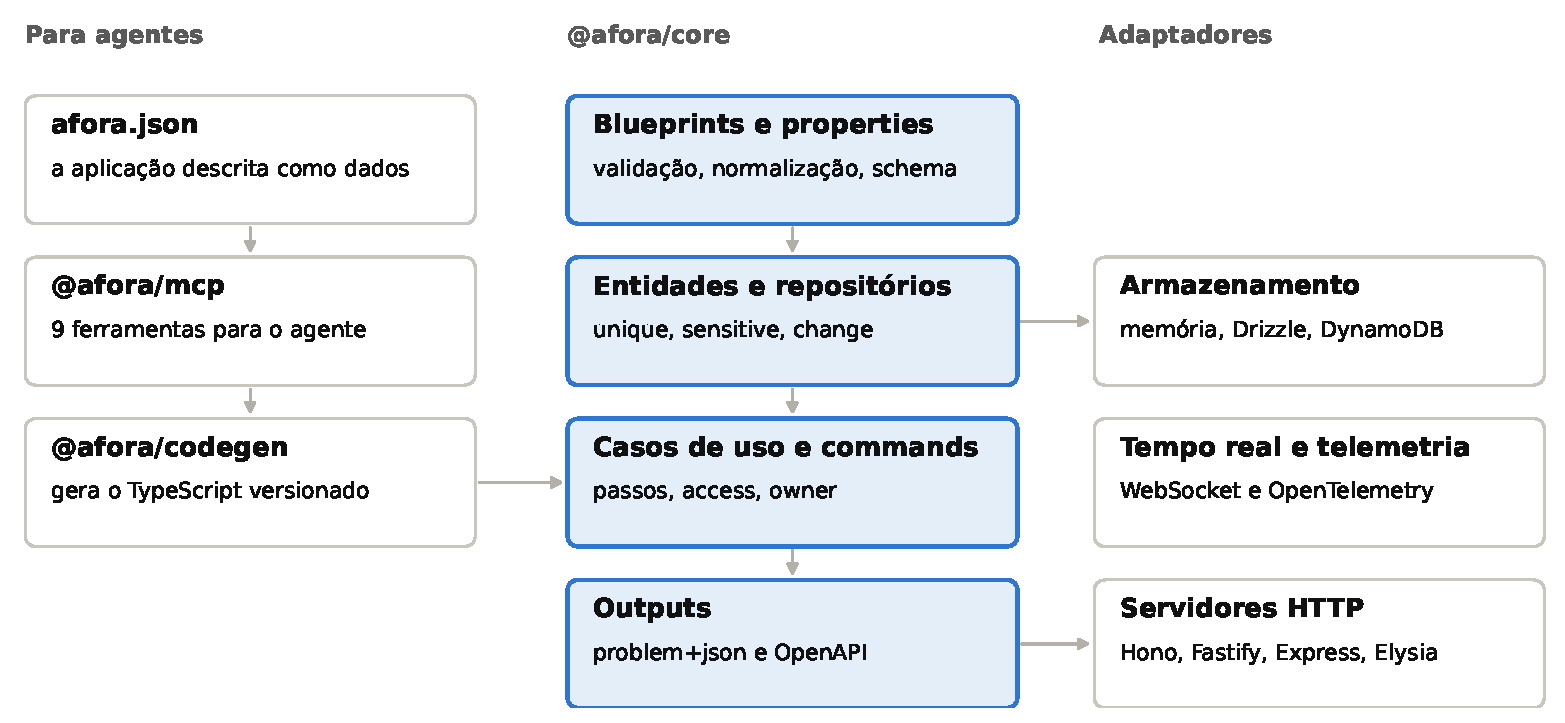
\includegraphics[width=.82\linewidth]{fig2.pdf}
\caption{Arquitetura do afora: núcleo, adaptadores e ferramentas para agentes.}\label{fig:arquitetura}
\fonte{elaborado pelo autor (2026).}
\end{figure}

\subsection{Garantias no \textit{runtime}}

A decisão de projeto mais importante foi mover para o \estr{runtime} garantias que, no Roastery, dependiam de \estr{plugins}. A Tabela~\ref{tab:garantias} as resume. A coluna ``Como vale'' separa dois tipos. As que valem \textbf{por padrão} não dependem de nenhuma linha da aplicação: um agente não tem como esquecê-las, só como contorná-las escrevendo código fora do caminho declarativo. As que valem \textbf{por declaração} são executadas pelo \estr{runtime}, mas só para o que o modelo declara. O \estr{framework} garante que a declaração será cumprida, não que ela será feita; o que muda é o lugar do esquecimento possível: uma linha do modelo, e não uma checagem em cada rota. As garantias foram escolhidas por dois critérios: corresponder a uma categoria da OWASP API Security Top 10 (última coluna) ou a uma falha observada no Roastery, onde o mascaramento e o mapeamento de erros dependiam de \estr{plugins}; a unicidade entra por ser a falha de integridade mais comum nos dois casos.

\begin{table}[!htb]
\centering
\caption{Garantias mantidas pelo \textit{runtime} do afora.}\label{tab:garantias}
\footnotesize
\renewcommand{\arraystretch}{1.1}
\begin{tabularx}{\linewidth}{>{\raggedright\arraybackslash}p{0.2\linewidth}>{\raggedright\arraybackslash}X>{\raggedright\arraybackslash}p{0.2\linewidth}>{\raggedright\arraybackslash}p{0.13\linewidth}}
\toprule
Falha comum & Garantia no afora & Como vale & OWASP \\
\midrule
\estr{Hash} ou \estr{token} numa resposta & Propriedades \texttt{sensitive} mascaradas pelo \texttt{toJSON()} em qualquer profundidade & Padrão na senha; declaração (\texttt{sensitive}) nos demais & API3 \\
Campos extras aceitos & Chaves não declaradas rejeitadas em qualquer profundidade (400) & Padrão & API3 \\
Erro de negócio vira 500 & Exceções conhecem a própria camada e viram \texttt{problem+json} com o status correto & Padrão; a camada de uma exceção própria é declarada & API8 \\
E-mail gravado duas vezes & Chaves \texttt{unique} garantidas pelo repositório (409) & Padrão em \texttt{ctx.slug} e no e-mail do \texttt{authenticatable}; declaração nos demais & -- \\
Usuário lê dados de outro & \texttt{access} (escopos, dono) verificado antes do caso de uso & Declaração (\texttt{access}, \texttt{owner}) por operação & API1 \\
Listagem sem limite & \texttt{limit} acima de \texttt{maxLimit} rejeitado (400) & Padrão & API4 \\
\bottomrule
\end{tabularx}
\fonte{elaborado pelo autor (2026), com base em OWASP (\citeyear{owasp2023}) e no código do afora.}
\end{table}

\subsection{A aplicação como dados}

Um arquivo \texttt{afora.json} declara entidades, casos de uso, \estr{commands} e a API HTTP. Casos de uso podem ser escritos como passos declarativos (\texttt{find}, \texttt{ensure}, \texttt{create}, \texttt{return}, entre outros), verificados pelo compilador. O pacote \path{@afora/mcp} expõe um servidor MCP com nove ferramentas para consultar o catálogo, editar e validar a especificação e gerar o código, e o \path{@afora/codegen} transforma a especificação no TypeScript que se escreveria à mão, com um caminho de volta que endereça o descompasso entre modelo e código \citep{hailpern2006}. Não há um \estr{runtime} paralelo: as garantias valem, pelo mesmo mecanismo, para o código escrito à mão e para o escrito pelo agente. Para que um \estr{framework} que promete garantias seja ele próprio confiável, o afora mantém um contrato público único (a partir da 27.0, quebras só no \estr{major} anual), passou por uma auditoria de segurança com 19 achados corrigidos e testados, e publica no npm com proveniência \citep{anjos2026tcc}.

% =====================================================================
\section{Avaliação}\label{sec:avaliacao}

\subsection{Volume de código}\label{sec:volume}

O mesmo CRUD de \estr{posts} foi contado em três formas (Tabela~\ref{tab:volume}): a cápsula do Roastery; o afora, com o \texttt{resourceOf}, que declara as cinco operações padrão de uma vez; e uma forma enxuta em Hono, Zod e Drizzle, sem DDD. As duas últimas foram escritas para esta avaliação e têm o mesmo comportamento, conferido por um roteiro de requisições (criar, ler, listar, alterar, apagar, 401, 400, 409 e 404).

\begin{table}[ht]
\centering
\caption{Volume de um mesmo CRUD de \textit{posts} em três formas.}\label{tab:volume}
\small
\renewcommand{\arraystretch}{1.1}
\begin{tabularx}{\linewidth}{>{\raggedright\arraybackslash}X rrr}
\toprule
Forma & Arquivos & Linhas não vazias & Caracteres\textsuperscript{a} \\
\midrule
Roastery, cápsula inteira (\texttt{b0c4f1f}) & 87 & 2.052 & 59.994 \\
Hono + Zod + Drizzle, enxuto & 1 & 80 & 4.055 \\
afora (quatro declarações e a aplicação) & 1 & 47 & 1.122 \\
\bottomrule
\end{tabularx}
\fonte{elaborado pelo autor com \path{tcc/metrics/count-volume.py}. \textsuperscript{a}Caracteres não brancos, medida que não depende da formatação.}
\end{table}

A comparação que importa é com a forma enxuta, e não com o Roastery, cuja arquitetura de microsserviços explica boa parte do volume: o afora usa 3,6 vezes menos caracteres. É uma comparação entre um recurso padrão declarado e um escrito à mão; geradores como o \estr{scaffold} do Rails também produzem um CRUD com poucos comandos, mas deixam o código no projeto, e essa comparação não foi medida. A redução não elimina código, ela o desloca: o núcleo do afora tem cerca de 39,5 mil linhas, escritas e testadas uma vez.

\subsection{Invariantes num \textit{backend} construído por agente}\label{sec:invariantes}

O exemplo \path{examples/agent-built} é uma avaliação de viabilidade: verifica se um agente que escreve um \estr{backend} apenas pelo servidor MCP chega a uma API que mantém as garantias do afora. O produto é um sistema de venda de ingressos, descrito em três versões de \estr{briefing} com o mesmo contrato HTTP: a~1 sem donos; a~2 com \estr{token}, eventos que só o organizador acessa e cada garantia enunciada como requisito; e a~3, igual à~2 mas sem listar as garantias, que é a que melhor testa a tese. Para as versões 1 e 2, um agente (Claude Opus 5.5, no Claude Code) produziu a especificação apenas via MCP, em 26 chamadas de ferramenta na versão~2; como linha de base, a mesma sessão escreveu uma implementação em Hono + Zod. A execução gravada foi a segunda passada: antes, a sessão já tinha escrito as verificações e ensaiado a especificação num rascunho.

Um roteiro percorre o contrato sobre a API em execução e verifica seis invariantes: as cinco primeiras da Tabela~\ref{tab:garantias} e uma regra de negócio, a capacidade sob compras simultâneas, que não é garantia do \estr{runtime}. Controles mostram que cada verificação pode falhar: uma API deliberadamente descuidada falha em todas, e uma que espera entre ler a capacidade e vender falha na de concorrência. A Tabela~\ref{tab:invariantes} mostra o resultado no \estr{briefing}~2; no~1, as invariantes aplicáveis também passaram nos dois lados.

\begin{table}[ht]
\centering
\caption{Invariantes verificadas no \textit{backend} construído por agente (\textit{briefing} 2, uma execução por lado).}\label{tab:invariantes}
\small
\renewcommand{\arraystretch}{1.1}
\begin{tabularx}{\linewidth}{>{\raggedright\arraybackslash}X ccc}
\toprule
Invariante & Verificações & afora & Linha de base \\
\midrule
Nenhum valor sensível em respostas & 45 & 45/45 & 45/45 \\
Chaves não declaradas rejeitadas & 5 & 5/5 & 5/5 \\
Erros como \texttt{problem+json}, nunca 5xx & 21 & 21/21 & 21/21 \\
Chaves únicas garantidas & 2 & 2/2 & 2/2 \\
Apenas o organizador acessa seu evento & 12 & 12/12 & 12/12 \\
\midrule
\multicolumn{4}{l}{\textit{Regra de negócio, declarada pelo agente em passos}} \\
Capacidade sob compras simultâneas & 5 & 5/5 & 5/5 \\
\bottomrule
\end{tabularx}
\fonte{elaborado pelo autor a partir de \path{examples/agent-built/eval/RESULTS.md} \citep{anjos2026afora}, reexecutado em 19/11/2026.}
\end{table}

As duas implementações passaram em tudo. Com uma execução por lado, a taxa de cada invariante é 1/1, cujo intervalo de Wilson a 95\% vai de 21\% a 100\%: o resultado mostra que o caminho funciona, não com que frequência, e não distingue os lados. A diferença está em como as garantias foram obtidas. No afora, nenhuma linha de implementação foi escrita para as cinco primeiras, mas elas ocupam 82 linhas de declaração, que também se revisam e podem estar erradas; a capacidade foi declarada em passos. A linha de base implementou cada garantia no próprio código: \texttt{.strict()} em cada \estr{schema}, remoção do \estr{hash} antes de cada resposta, tratamento próprio de erros, mapas para unicidade, verificação de \estr{token} e uma checagem de dono em cada rota. Com armazenamento síncrono em memória, a invariante de concorrência tende a passar nos dois lados.

O repositório contém um \estr{script} que faz $N$ execuções independentes por modelo, \estr{briefing} e lado, que é o que compararia agentes com e sem o afora. O lote não foi executado por falta de recursos para custear o uso da API: a configuração mínima útil, com dez execuções por lado no \estr{briefing}~3, exige cerca de 330 requisições e 22 milhões de \estr{tokens} de entrada, segundo a estimativa do próprio \estr{script}, e o trabalho não teve financiamento. Uma execução manual do \estr{briefing}~3 teria $n = 1$ e a mesma contaminação da linha de base, e por isso também não foi feita.

\subsection{Custo de revisão}\label{sec:revisao}

Para medir o tamanho do que se revisa, cada linha da linha de base e do \texttt{afora.json} do \estr{briefing}~2 foi atribuída a uma garantia ou a nenhuma, numa classificação versionada que qualquer pessoa pode contestar (\path{tcc/metrics/review-cost.classes.json}). Como o \texttt{afora.json} tem um valor por linha, a Tabela~\ref{tab:revisao} também traz os caracteres não brancos.

\begin{table}[ht]
\centering
\caption{Linhas e caracteres dedicados a cada garantia (\textit{briefing} 2).}\label{tab:revisao}
\small
\renewcommand{\arraystretch}{1.1}
\begin{tabularx}{\linewidth}{>{\raggedright\arraybackslash}X rrrr}
\toprule
 & \multicolumn{2}{c}{Linha de base} & \multicolumn{2}{c}{afora (\texttt{afora.json})} \\
Garantia & Linhas & Caracteres & Linhas & Caracteres \\
\midrule
Chaves não declaradas & 5 & 50 & 0 & 0 \\
Valores sensíveis & 4 & 168 & 3 & 29 \\
Erros em \texttt{problem+json} & 58 & 1.285 & 28 & 479 \\
Chaves únicas & 18 & 379 & 1 & 14 \\
\estr{Token} e dono & 55 & 1.587 & 50 & 500 \\
Capacidade & 6 & 201 & 19 & 204 \\
\midrule
Total das garantias & 146 & 3.670 & 101 & 1.226 \\
\bottomrule
\end{tabularx}
\fonte{elaborado pelo autor com \path{tcc/metrics/review-cost.ts}; linhas não vazias.}
\end{table}

O resultado é mais modesto que a tese sugeria. Em caracteres, as garantias ocupam três vezes menos no afora, e quatro delas quase desaparecem. Mas a de \estr{token} e dono, a mais importante para a OWASP, ocupa quase o mesmo número de linhas (50 contra 55), porque o \texttt{afora.json} repete \texttt{access} e \texttt{owner} em cada operação, e a capacidade custa mais, porque foi declarada em passos. A diferença que a tabela não capta é de natureza: as linhas do afora dizem quem é o dono; as da linha de base implementam a verificação, e cada uma pode estar errada. O tempo efetivo de revisão não foi medido.

\subsection{Desempenho e uso real}\label{sec:desempenho}

Garantias no \estr{runtime} têm custo. Nos \estr{benchmarks} versionados, que comparam o afora com nove bibliotecas sob as mesmas regras, a validação pura do afora ficou na faixa das mais usadas e, na maioria dos cenários, à frente do Zod. O caminho real de uma requisição, que constrói a entidade, levou de 1,9 a 2,7 vezes o tempo do Zod num objeto pequeno, e até 5,7 vezes sem transformação, em Bun e Node.js. Em escala, a requisição completa, sem rede, ficou entre 0,2 e 0,5~ms na mediana, de 1,6 a 6,3 vezes a forma enxuta, com armazenamentos diferentes nos dois lados \citep{anjos2026tcc}.

O afora roda em dois sistemas do autor, ambos escritos em grande parte com agentes. No CMS do \estr{site} do afora, o sistema usa o núcleo, mas não a saída HTTP, e três garantias voltam a ser código da aplicação. Na API do \estr{site} pessoal \citep{anjos2026site}, refeita sobre o afora, o código cresceu 27\%: lá não há um CRUD padrão, e sim casos de uso com regras próprias e um provedor de armazenamento que o afora não tinha. Repositórios e serviços viraram declarações, mas a unicidade passou a depender desse provedor, e um defeito nele só foi encontrado na revisão.

% =====================================================================
\section{Discussão}\label{sec:discussao}

O argumento do trabalho é que o \estr{AI slop} resulta da assimetria entre gerar e verificar, e que \estr{frameworks} podem reduzi-la diminuindo o que precisa ser verificado. Os resultados sustentam parte dele. Uma garantia que vale por padrão não tem linha em que possa ser esquecida, e Finifter e Wagner (\citeyear{finifter2011}) mostram que proteções automáticas funcionam onde as manuais falham; no experimento, as cinco garantias se mantiveram sem implementação, contra 140 linhas de código na linha de base (Tabela~\ref{tab:revisao}, sem a capacidade). O texto que o revisor lê encolhe três vezes em caracteres, e a pergunta dele muda de ``o que foi esquecido em cada \estr{handler}?'' para ``o modelo e as declarações estão certos?''. O que o trabalho não mostra é que um agente sem o afora esqueceria as garantias: na única execução, ele não esqueceu.

\subsection{Os limites da tese}\label{sec:limites}

O primeiro limite está dentro das próprias garantias: as que valem por declaração só protegem o que foi declarado. Um agente que esquece o \texttt{owner} de uma operação produz uma rota que qualquer usuário autenticado alcança. A omissão fica visível no modelo, e a ferramenta \texttt{afora\_project} aponta operações sem acesso declarado ao lado de outras que o declaram; ela não aponta, porém, uma operação com \texttt{access} e sem \texttt{owner}, nem uma aplicação em que nenhuma operação declara acesso. Além disso, o afora não impede um agente de modelar mal o domínio. A autorização rica (papéis, permissões que dependem do estado, regras entre entidades) fica no código do caso de uso, assim como os adaptadores que a aplicação escreve, como mostrou o provedor do \estr{site} pessoal. Como alertam Weinberger \etal{} (\citeyear{weinberger2011}), a automação protege apenas o que cobre. A tese, portanto, não é que o afora elimina o \estr{slop}, mas que o empurra para onde a revisão humana é insubstituível: o modelo e as regras do negócio, onde os LLMs se mostraram mais fracos \citep{camara2023}.

\subsection{Ameaças à validade}

O pesquisador é o desenvolvedor do artefato, e o relato das gerações anteriores é retrospectivo. O experimento tem uma execução por lado, e o \estr{briefing}~3 não tem resultados. Os dois lados estão contaminados: a linha de base foi escrita pela mesma sessão que acabara de escrever as verificações, a partir de um \estr{briefing} que enumerava as garantias, e o lado do afora teve ainda um ensaio prévio. O mesmo modelo construiu o experimento, escreveu os CRUDs da Tabela~\ref{tab:volume}, classificou as linhas da Tabela~\ref{tab:revisao} e ajudou a redigir o texto; por isso, todo número vem de um \estr{script} versionado e reexecutável. O custo de revisão foi medido em linhas e caracteres, não em tempo. O uso real é do próprio autor, e a evidência vem de domínios simples; regras de negócio mais ricas podem exigir mais código fora das declarações.

% =====================================================================
\section{Conclusão}\label{sec:conclusao}

Este trabalho apresentou o afora, um \estr{framework} para \estr{backends} em TypeScript que mantém no \estr{runtime} garantias que, em outras ferramentas, dependem de quem escreve a aplicação. O objetivo geral foi atingido no que diz respeito ao artefato: o produto está publicado, em \estr{release candidate} da primeira versão estável, e mantém invariantes de segurança e consistência, parte por padrão e parte a partir de declarações do modelo. As garantias foram identificadas na literatura e na experiência com o Roastery (objetivo~1); a \estr{blueprint} passou a ser a fonte única do modelo (objetivo~2); as garantias viraram comportamento do \estr{runtime} (objetivo~3); e a aplicação pode ser descrita em \texttt{afora.json} e escrita por agentes via MCP (objetivo~4). Na avaliação (objetivo~5), um CRUD padrão coube em 3,6 vezes menos caracteres que uma forma enxuta; um agente construiu pelo MCP um \estr{backend} que manteve as garantias, assim como a linha de base; o texto dedicado às garantias encolheu três vezes, mas não o da autorização; e construir entidades pequenas custou várias vezes o tempo do Zod.

A trajetória do produto mostra três deslocamentos: de cerimônia a declaração, de convenção a garantia e de quarenta repositórios a um contrato. A contribuição central é um princípio de projeto, apoiado por trabalhos anteriores sobre proteções automáticas em \estr{frameworks} web: \textbf{o que não pode ser esquecido não deve depender de ser lembrado}. Saber se esse princípio torna o código de agentes mais seguro na prática exige uma avaliação em lote, cujo protocolo já está pronto. Como trabalhos futuros, propõem-se: executar esse lote, com o \estr{briefing}~3 e uma linha de base escrita sem acesso às verificações; transformar em avisos da especificação as declarações que um agente pode esquecer, como uma operação sem \texttt{owner}; conduzir um estudo com desenvolvedores externos, medindo tempo de construção, defeitos e tempo de revisão; reduzir o custo de construção de entidades; e avaliar o \estr{framework} em domínios com regras de negócio e de autorização mais ricas.

% =====================================================================
\section*{Declaração de Uso de Inteligência Artificial}

Conforme a Portaria CNPq nº 2.664/2026 e o Art. 12 das Normas de TCC, declara-se o uso das seguintes ferramentas de IA generativa:
\begin{enumerate}
  \item \textbf{Desenvolvimento do produto.} Claude Code (Anthropic), com os modelos Claude Opus 5.5, Claude Fable 5.2 e Claude Sonnet 5.5, e Codex (OpenAI). Finalidade: escrever, sob a direção e a revisão do autor, parte do código-fonte, dos testes e da documentação do afora; dos 577 \estr{commits} entre 5 e 18 de novembro de 2026, 388 têm coautoria de um modelo Claude e 9 do Codex.
  \item \textbf{Redação e revisão do texto.} Claude (Anthropic), modelo Claude Opus 5.5. Finalidades: estruturar e redigir versões do texto a partir de um texto-base do autor, conferir referências e afirmações contra o código e as fontes, montar o arquivo \LaTeX{} no modelo da SBC e reduzir o texto ao limite das Normas.
  \item \textbf{Medições e avaliação.} Claude Opus 5.5, no Claude Code e no Claude. Finalidades: escrever e executar os \estr{scripts} de \path{tcc/metrics/}, as formas de CRUD da Tabela~\ref{tab:volume} e a classificação da Tabela~\ref{tab:revisao}, e construir, como objeto do experimento, o \estr{backend} e a linha de base da Seção~\ref{sec:invariantes}.
\end{enumerate}
Todo número citado vem de um arquivo versionado e reexecutável, e os resultados desfavoráveis foram mantidos. O autor é responsável pelo conteúdo final do trabalho.

% =====================================================================
\renewcommand{\refname}{Referências}
\begin{thebibliography}{99}
\small
\setlength{\itemsep}{2pt}

\bibitem[{Amplication}(2026)]{amplication2026}
AMPLICATION. \textbf{Amplication}: open-source backend development platform. [\textit{S. l.}]: GitHub, 2026. Disponível em: \url{https://github.com/amplication/amplication}. Acesso em: 22 nov. 2026.

\bibitem[{Anjos}(2026a)]{anjos2026afora}
ANJOS, A. R. \textbf{afora}: simple to write, built to hold. Versão 27.0.0-rc.4. [\textit{S. l.}]: GitHub, 16 nov. 2026. Disponível em: \url{https://github.com/afora-framework/core}. Acesso em: 19 nov. 2026.

\bibitem[{Anjos}(2026b)]{anjos2026roastery}
ANJOS, A. R. \textbf{Roastery CMS}: repositórios da organização roastery-cms. [\textit{S. l.}]: GitHub, 2026. Disponível em: \url{https://github.com/roastery-cms}. Acesso em: 19 nov. 2026.

\bibitem[{Anjos}(2026c)]{anjos2026site}
ANJOS, A. R. \textbf{hoyasumii.dev}: portfólio e painel de conteúdo. [\textit{S. l.}]: GitHub, 2026. Disponível em: \url{https://github.com/Hoyasumii/Hoyasumii}. Acesso em: 22 nov. 2026.

\bibitem[{Anjos}(2026d)]{anjos2026tcc}
ANJOS, A. R. \textbf{Da cerimônia à declaração}: o afora e as garantias de \textit{runtime} para \textit{backends} TypeScript escritos por pessoas e agentes de IA. Relatório técnico (versão estendida). Aracaju: Universidade Tiradentes, 2026. Disponível em: \url{https://github.com/Hoyasumii/tcc-afora}. Acesso em: 23 nov. 2026.

\bibitem[{Ash}(2026)]{ash2026}
ASH FRAMEWORK. \textbf{What is Ash?}. Documentação oficial. [\textit{S. l.}], 2026. Disponível em: \url{https://hexdocs.pm/ash/what-is-ash.html}. Acesso em: 22 nov. 2026.

\bibitem[{Becker \etal}(2025)]{becker2025}
BECKER, J. \textit{et al.} \textbf{Measuring the impact of early-2025 AI on experienced open-source developer productivity}. [\textit{S. l.}]: arXiv, 2025. Preprint arXiv:2507.09089. Disponível em: \url{https://arxiv.org/abs/2507.09089}. Acesso em: 18 nov. 2026.

\bibitem[{Brooks}(1987)]{brooks1987}
BROOKS, F. P. No silver bullet: essence and accidents of software engineering. \textbf{Computer}, v. 20, n. 4, p. 10--19, abr. 1987. DOI: 10.1109/MC.1987.1663532.

\bibitem[{Burket \etal}(2011)]{burket2011}
BURKET, J.; MUTCHLER, P.; WEAVER, M.; ZAVERI, M.; EVANS, D. GuardRails: a data-centric web application security framework. \textit{In}: USENIX CONFERENCE ON WEB APPLICATION DEVELOPMENT (WebApps '11), 2., 2011, Portland. \textbf{Proceedings} [...]. Berkeley: USENIX Association, 2011. Disponível em: \url{https://www.usenix.org/conference/webapps11/guardrails-data-centric-web-application-security-framework}. Acesso em: 19 nov. 2026.

\bibitem[{Cámara \etal}(2023)]{camara2023}
CÁMARA, J.; TROYA, J.; BURGUEÑO, L.; VALLECILLO, A. On the assessment of generative AI in modeling tasks: an experience report with ChatGPT and UML. \textbf{Software and Systems Modeling}, v. 22, n. 3, p. 781--793, 2023. DOI: 10.1007/s10270-023-01105-5.

\bibitem[{Drowning\ldots}(2026)]{newstack2026}
DROWNING in AI slop, cURL ends bug bounties. \textbf{The New Stack}, [\textit{S. l.}], 22 jan. 2026. Disponível em: \url{https://thenewstack.io/drowning-in-ai-slop-reports-curl-ends-bug-bounties/}. Acesso em: 18 nov. 2026.

\bibitem[{Evans}(2004)]{evans2004}
EVANS, E. \textbf{Domain-driven design}: tackling complexity in the heart of software. Boston: Addison-Wesley, 2004.

\bibitem[{Finifter; Wagner}(2011)]{finifter2011}
FINIFTER, M.; WAGNER, D. Exploring the relationship between web application development tools and security. \textit{In}: USENIX CONFERENCE ON WEB APPLICATION DEVELOPMENT (WebApps '11), 2., 2011, Portland. \textbf{Proceedings} [...]. Berkeley: USENIX Association, 2011. Disponível em: \url{https://www.usenix.org/conference/webapps11/exploring-relationship-between-web-application-development-tools-and-security}. Acesso em: 19 nov. 2026.

\bibitem[{Hailpern; Tarr}(2006)]{hailpern2006}
HAILPERN, B.; TARR, P. Model-driven development: the good, the bad, and the ugly. \textbf{IBM Systems Journal}, v. 45, n. 3, p. 451--461, 2006. DOI: 10.1147/sj.453.0451.

\bibitem[{Hevner \etal}(2004)]{hevner2004}
HEVNER, A. R. \textit{et al.} Design science in information systems research. \textbf{MIS Quarterly}, v. 28, n. 1, p. 75--105, 2004. DOI: 10.2307/25148625.

\bibitem[{JHipster}(2026)]{jhipster2026}
JHIPSTER. \textbf{Creating an entity}. Documentação oficial. [\textit{S. l.}], 2026. Disponível em: \url{https://www.jhipster.tech/creating-an-entity/}. Acesso em: 19 nov. 2026.

\bibitem[{Karpathy}(2025)]{karpathy2025}
KARPATHY, A. [Postagem que introduz o termo ``vibe coding'']. [\textit{S. l.}], fev. 2025. X: @karpathy. Disponível em: \url{https://x.com/karpathy/status/1886192184808149383}. Acesso em: 18 nov. 2026.

\bibitem[{King}(2019)]{king2019}
KING, A. \textbf{Parse, don't validate}. [\textit{S. l.}], 5 nov. 2019. Disponível em: \url{https://lexi-lambda.github.io/blog/2019/11/05/parse-don-t-validate/}. Acesso em: 18 nov. 2026.

\bibitem[{Martin}(2018)]{martin2018}
MARTIN, R. C. \textbf{Clean architecture}: a craftsman's guide to software structure and design. Boston: Prentice Hall, 2018.

\bibitem[{Mündler \etal}(2025)]{mundler2025}
MÜNDLER, N.; HE, J.; WANG, H.; SEN, K.; SONG, D.; VECHEV, M. Type-constrained code generation with language models. \textbf{Proceedings of the ACM on Programming Languages}, v. 9, n. PLDI, p. 601--626, 2025. DOI: 10.1145/3729274.

\bibitem[{NestJS}(2026)]{nestjs2026}
NESTJS. \textbf{Validation}. Documentação oficial. [\textit{S. l.}], 2026. Disponível em: \url{https://docs.nestjs.com/techniques/validation}. Acesso em: 19 nov. 2026.

\bibitem[{Nottingham; Wilde; Dalal}(2023)]{rfc9457}
NOTTINGHAM, M.; WILDE, E.; DALAL, S. \textbf{RFC 9457}: problem details for HTTP APIs. [\textit{S. l.}]: IETF, jul. 2023. DOI: 10.17487/RFC9457.

\bibitem[{OWASP}(2023)]{owasp2023}
OWASP. \textbf{OWASP API Security Top 10 -- 2023}. [\textit{S. l.}]: OWASP Foundation, 2023. Disponível em: \url{https://api-security.owasp.org/editions/2023/en/0x11-t10/}. Acesso em: 18 nov. 2026.

\bibitem[{Pearce \etal}(2022)]{pearce2022}
PEARCE, H. \textit{et al.} Asleep at the keyboard? Assessing the security of GitHub Copilot's code contributions. \textit{In}: IEEE SYMPOSIUM ON SECURITY AND PRIVACY, 2022. \textbf{Proceedings} [...]. [\textit{S. l.}]: IEEE, 2022. p. 754--768. DOI: 10.1109/SP46214.2022.9833571.

\bibitem[{Peffers \etal}(2007)]{peffers2007}
PEFFERS, K. \textit{et al.} A design science research methodology for information systems research. \textbf{Journal of Management Information Systems}, v. 24, n. 3, p. 45--77, 2007. DOI: 10.2753/MIS0742-1222240302.

\bibitem[{Peng \etal}(2023)]{peng2023}
PENG, S. \textit{et al.} \textbf{The impact of AI on developer productivity}: evidence from GitHub Copilot. [\textit{S. l.}]: arXiv, 2023. Preprint arXiv:2302.06590. Disponível em: \url{https://arxiv.org/abs/2302.06590}. Acesso em: 18 nov. 2026.

\bibitem[{Perry \etal}(2023)]{perry2023}
PERRY, N. \textit{et al.} Do users write more insecure code with AI assistants? \textit{In}: ACM SIGSAC CONFERENCE ON COMPUTER AND COMMUNICATIONS SECURITY, 2023, Copenhagen. \textbf{Proceedings} [...]. New York: ACM, 2023. p. 2785--2799. DOI: 10.1145/3576915.3623157.

\bibitem[{Poesia \etal}(2022)]{poesia2022}
POESIA, G.; POLOZOV, O.; LE, V.; TIWARI, A.; SOARES, G.; MEEK, C.; GULWANI, S. Synchromesh: reliable code generation from pre-trained language models. \textit{In}: INTERNATIONAL CONFERENCE ON LEARNING REPRESENTATIONS, 2022. \textbf{Proceedings} [...]. [\textit{S. l.}]: ICLR, 2022. Disponível em: \url{https://arxiv.org/abs/2201.11227}. Acesso em: 19 nov. 2026.

\bibitem[{PostgREST}(2026)]{postgrest2026}
POSTGREST. \textbf{PostgREST}: REST API for any Postgres database. [\textit{S. l.}]: GitHub, 2026. Disponível em: \url{https://github.com/PostgREST/postgrest}. Acesso em: 19 nov. 2026.

\bibitem[{Ruby on Rails}(2026)]{rails2026}
RUBY ON RAILS. \textbf{Active Record Validations}. Rails Guides, v. 8.1. [\textit{S. l.}], 2026. Disponível em: \url{https://guides.rubyonrails.org/active_record_validations.html}. Acesso em: 19 nov. 2026.

\bibitem[{Stenberg}(2026)]{stenberg2026}
STENBERG, D. \textbf{The end of the curl bug-bounty}. [\textit{S. l.}], 26 jan. 2026. Disponível em: \url{https://daniel.haxx.se/blog/2026/01/26/the-end-of-the-curl-bug-bounty/}. Acesso em: 18 nov. 2026.

\bibitem[{TypeBox}(2026)]{typebox2026}
TYPEBOX. \textbf{TypeBox}: JSON Schema type builder with static type resolution for TypeScript. [\textit{S. l.}]: GitHub, 2026. Disponível em: \url{https://github.com/sinclairzx81/typebox}. Acesso em: 23 nov. 2026.

\bibitem[{Venable; Pries-Heje; Baskerville}(2016)]{venable2016}
VENABLE, J.; PRIES-HEJE, J.; BASKERVILLE, R. FEDS: a framework for evaluation in design science research. \textbf{European Journal of Information Systems}, v. 25, n. 1, p. 77--89, 2016. DOI: 10.1057/ejis.2014.36.

\bibitem[{Vero \etal}(2025)]{vero2025}
VERO, M.; MÜNDLER, N.; CHIBOTARU, V.; RAYCHEV, V.; BAADER, M.; JOVANOVIĆ, N.; HE, J.; VECHEV, M. BaxBench: can LLMs generate correct and secure backends? \textit{In}: INTERNATIONAL CONFERENCE ON MACHINE LEARNING, 42., 2025, Vancouver. \textbf{Proceedings} [...]. [\textit{S. l.}]: PMLR, 2025. (Proceedings of Machine Learning Research, v. 267). Disponível em: \url{https://arxiv.org/abs/2502.11844}. Acesso em: 19 nov. 2026.

\bibitem[{Weinberger \etal}(2011)]{weinberger2011}
WEINBERGER, J.; SAXENA, P.; AKHAWE, D.; FINIFTER, M.; SHIN, R.; SONG, D. A systematic analysis of XSS sanitization in web application frameworks. \textit{In}: ATLURI, V.; DIAZ, C. (ed.). \textbf{Computer Security -- ESORICS 2011}. Berlin, Heidelberg: Springer, 2011. p. 150--171. (Lecture Notes in Computer Science, v. 6879). DOI: 10.1007/978-3-642-23822-2\_9.

\bibitem[{Willison}(2024)]{willison2024}
WILLISON, S. \textbf{Slop is the new name for unwanted AI-generated content}. [\textit{S. l.}], 8 maio 2024. Disponível em: \url{https://simonwillison.net/2024/May/8/slop/}. Acesso em: 18 nov. 2026.

\bibitem[{Zod}(2026)]{zod2026}
ZOD. \textbf{Defining schemas}. Documentação oficial da API. [\textit{S. l.}], 2026. Disponível em: \url{https://zod.dev/api}. Acesso em: 19 nov. 2026.

\end{thebibliography}

\end{document}
